\documentclass[12pt,a4paper]{report}
\setlength\textwidth{160mm}
\setlength\textheight{247mm}
\setlength\oddsidemargin{0mm}
\setlength\evensidemargin{0mm}
\setlength\topmargin{0mm}
\setlength\headsep{0mm}
\setlength\headheight{0mm}
% \openright makes the following text appear on a right-hand page
\let\openright=\clearpage

%% Generate PDF/A-2u
\usepackage[a-2u]{pdfx}

%% Character encoding: usually latin2, cp1250 or utf8:
\usepackage[utf8]{inputenc}

%% Prefer Latin Modern fonts
\usepackage{lmodern}

%% Further useful packages (included in most LaTeX distributions)
\usepackage{amsmath}        % extensions for typesetting of math
\usepackage{amsfonts}       % math fonts
\usepackage{amsthm}         % theorems, definitions, etc.
\usepackage{bbding}         % various symbols (squares, asterisks, scissors, ...)
\usepackage{bm}             % boldface symbols (\bm)
\usepackage{graphicx}       % embedding of pictures
\usepackage{fancyvrb}       % improved verbatim environment
\usepackage{natbib}         % citation style AUTHOR (YEAR), or AUTHOR [NUMBER]
\usepackage[nottoc]{tocbibind} % makes sure that bibliography and the lists
			    % of figures/tables are included in the table
			    % of contents
\usepackage{dcolumn}        % improved alignment of table columns
\usepackage{booktabs}       % improved horizontal lines in tables
\usepackage{paralist}       % improved enumerate and itemize
\usepackage{xcolor}         % typesetting in color

\usepackage{tikz-qtree}
\usepackage{array}
\usepackage{multicol}
\usepackage[ruled,vlined,linesnumbered]{algorithm2e}

\usetikzlibrary{shapes.geometric}
\usetikzlibrary{positioning}
\tikzset{every tree node/.style={minimum size=7mm,draw,circle},
         blank/.style={draw=none},
         edge from parent path={(\tikzparentnode)--(\tikzchildnode)},
         level distance=1.2cm,
         triangle/.style={regular polygon, regular polygon sides=3},
         tosubtree/.style={edge from parent path={(\tikzparentnode)--(\tikzchildnode.north)}},
         }


%%% Basic information on the thesis

\def\ThesisTitle{Persistent Weak-AVL Trees}

\def\ThesisAuthor{Jiří Škrobánek}

\def\YearSubmitted{2021}

\def\Department{Department of Applied Mathematics}

\def\DeptType{Department}

% Thesis supervisor: name, surname and titles
\def\Supervisor{Mgr. Martin Mareš, Ph.D.}

% Supervisor's department (again according to Organizational structure of MFF)
\def\SupervisorsDepartment{Department of Applied Mathematics}

% Study programme and specialization
\def\StudyProgramme{Computer Science}
\def\StudyBranch{General Computer Science}

\def\Dedication{%
\vspace{50mm}

\noindent
I hereby express many thanks to my supervisor Martin Mareš for guiding me through the labyrinth of algorithms and data structures.
}

\def\Abstract{%
This thesis investigates persistence (i.e., preservation of data by updates) of binary search trees. 
In particular, we explore how weak-AVL trees may be converted into efficient fully-persistent data structures.
After mentioning all important properties of weak-AVL trees, we present a new method to store them with worst-case constant number of changes per update. 
Then we show some general schemes for conversion of binary search trees (and possibly other pointer-based data structures) into their persistent variants. 
Finally the established theory is used to obtain fully-persistent weak-AVL trees.
}

% 3 to 5 keywords (recommended), each enclosed in curly braces
\def\Keywords{%
{Persistence} {Weak-AVL trees} {Rank-balanced trees}
}

%% The hyperref package for clickable links in PDF and also for storing
%% metadata to PDF (including the table of contents).
%% Most settings are pre-set by the pdfx package.
\hypersetup{unicode}
\hypersetup{breaklinks=true}

% Definitions of macros (see description inside)
%%% This file contains definitions of various useful macros and environments %%%
%%% Please add more macros here instead of cluttering other files with them. %%%

%%% Minor tweaks of style

% These macros employ a little dirty trick to convince LaTeX to typeset
% chapter headings sanely, without lots of empty space above them.
% Feel free to ignore.
\makeatletter
\def\@makechapterhead#1{
  {\parindent \z@ \raggedright \normalfont
   \Huge\bfseries \thechapter. #1
   \par\nobreak
   \vskip 20\p@
}}
\def\@makeschapterhead#1{
  {\parindent \z@ \raggedright \normalfont
   \Huge\bfseries #1
   \par\nobreak
   \vskip 20\p@
}}
\makeatother

% This macro defines a chapter, which is not numbered, but is included
% in the table of contents.
\def\chapwithtoc#1{
\chapter*{#1}
\addcontentsline{toc}{chapter}{#1}
}

% Draw black "slugs" whenever a line overflows, so that we can spot it easily.
\overfullrule=1mm

%%% Macros for definitions, theorems, claims, examples, ... (requires amsthm package)

\newtheoremstyle{mytheoremstyle} % name
{\topsep}                    % Space above
{\topsep}                    % Space below
{\slshape}                   % Body font
{}                           % Indent amount
{\bfseries}                   % Theorem head font
{.}                          % Punctuation after theorem head
{.5em}                       % Space after theorem head
{}  % Theorem head spec (can be left empty, meaning ‘normal’)

\theoremstyle{mytheoremstyle}
\newtheorem{thm}{Theorem}
\newtheorem{lemma}[thm]{Lemma}
\newtheorem{claim}[thm]{Claim}
\newtheorem{prop}[thm]{Proposition}

\theoremstyle{mytheoremstyle}
\newtheorem{defn}{Definition}

\theoremstyle{remark}
\newtheorem*{cor}{Corollary}
\newtheorem*{obs}{Observation}
\newtheorem*{rem}{Remark}
\newtheorem*{example}{Example}

%%% An environment for proofs

\newenvironment{myproof}{
  \par\medskip\noindent
  \textit{Proof}.
}{
\newline
\rightline{$\qedsymbol$}
}

%%% An environment for typesetting of program code and input/output
%%% of programs. (Requires the fancyvrb package -- fancy verbatim.)

\DefineVerbatimEnvironment{code}{Verbatim}{fontsize=\small, frame=single}

%%% The field of all real and natural numbers
\newcommand{\R}{\mathbb{R}}
\newcommand{\N}{\mathbb{N}}

%%% Useful operators for statistics and probability
\DeclareMathOperator{\pr}{\textsf{P}}
\DeclareMathOperator{\E}{\textsf{E}\,}
\DeclareMathOperator{\var}{\textrm{var}}
\DeclareMathOperator{\sd}{\textrm{sd}}

%%% Transposition of a vector/matrix
\newcommand{\T}[1]{#1^\top}

%%% Various math goodies
\newcommand{\goto}{\rightarrow}
\newcommand{\gotop}{\stackrel{P}{\longrightarrow}}
\newcommand{\maon}[1]{o(n^{#1})}
\newcommand{\abs}[1]{\left|{#1}\right|}
\newcommand{\dint}{\int_0^\tau\!\!\int_0^\tau}
\newcommand{\isqr}[1]{\frac{1}{\sqrt{#1}}}

%%% Various table goodies
\newcommand{\pulrad}[1]{\raisebox{1.5ex}[0pt]{#1}}
\newcommand{\mc}[1]{\multicolumn{1}{c}{#1}}

\newcommand{\bigO}[1]{$\mathcal{O}(#1)$}

\newenvironment{vdTable}[1]{
\begin{tabular}{|m{0.085\textwidth} m{0.06\textwidth} m{0.06\textwidth} m{0.06\textwidth} m{0.06\textwidth}|}
\hline
\bfseries #1 & & & & \\
}{
\\ \hline
	\end{tabular}
}

%https://tex.stackexchange.com/questions/12703/how-to-create-fixed-width-table-columns-with-text-raggedright-centered-raggedlef

% Mathmode slanted:

\def\leftit{\text{\it left}}
\def\rightit{\text{\it right}}
\def\sizeit{\text{\it size}}
\def\weightit{\text{\it weight}}
\def\keyit{\text{\it key}}
\def\rank{\text{\it rank}}

% Title page and various mandatory informational pages
\begin{document}
\include{title}

\tableofcontents

\chapter*{Introduction}
\addcontentsline{toc}{chapter}{Introduction}

This thesis strives to enhance the existing knowledge of persistent data structures, predominantly we will seek to use weak-AVL trees to construct fully-persistent binary search trees.

Speaking in general terms, persistent data structures maintain their previous versions when modified. Operations can thus also be executed on any earlier state of the structure. When such an operation updates the structure, a new version is created branching out of the original sequence of updates.

Use of term \emph{persistent} was introduced by Driscoll, Sarnak, Sleator, and Tarjan in their joint 1986 article \emph{Making data structures persistent} \cite{persistence-DSST}. It turned out that much more efficient algorithms than copying the whole data structure are attainable. In this article a general scheme for converting regular pointer-based data structures into persistent ones is given. Persistent binary search tree was constructed from adapted Red-Black trees.

Haeupler, Sen, and Tarjan \cite{weight-balanced} introduced weak-AVL (WAVL) trees as part of a framework of rank balanced trees in 2015. WAVL trees were named after AVL trees which form a subset of them.

The algorithms for WAVL operations given by Haeupler at al. cannot be directly plugged into the persistence scheme by Driscoll at al. Modifications are needed alike those done to red-black trees during their conversion into persistent binary search trees. These modifications are the main topic in this thesis. The structure of the binary tree remains unmodified, the method of storing ranks must undergo considerable changes however.

We also describe a variant of persistent WAVL trees which supports queries on earlier versions and is suitable for concurrent operations.

We begin the thesis by swiftly establishing fundamentals of binary search trees. These topics are covered in Chapter 1. Chapter 2 moves to construct our modification of WAVL trees suitable for persistence. Several approaches to persistence of binary search trees are described in Chapter 3. A structure for handling versions as elements of an ordering is also covered. Persistent data structures were motivated by many direct and obscured applications, we mention some of them in Chapter 4. Implementation of persistent WAVL trees is the focus of Chapter 5.

% Since the original publication on persistence great number of other works addressing this topic appeared.

\chapter{Binary Search Trees Data Structures}

In this chapter basic terminology concerning trees will be established. Then a quick review of Weak-AVL (WAVL) trees is given. Next, our modified balancing algorithm is introduced. Finally, weight-balanced trees are defined since these will be needed as an auxiliary structure in persistent BSTs.

\section{Terminology}

For the purposes of this thesis, \emph{binary search tree} (BST) will be a data structure composed of internal vertices (or nodes). Every internal vertex carries a key. Keys are members of a set of linearly ordered items and naturally extend this ordering to vertices. In addition, internal vertices are allowed to carry constant amount of information in fields (for example about tree structure) and to have constant number of pointers to other vertices. An internal node has two pointers to child vertices -- left and right. Any of the pointers can target an external vertex. 

External vertices are not represented in memory, all pointers (null-pointers) to external vertices are equal and must not be dereferenced. For the specific application, it can be beneficial to assume external vertices have some default values of their fields. An internal left child must precede its parent in the linear order, conversely an internal right child must come after its parent in the linear order.

Binary search trees naturally represent finite rooted ordered (i.e. order of children is also relevant) trees where every vertex has degree at most three and the root has degree at most two.

When we work with binary search trees, we typically use a specific algorithm that only accepts a specific subclass of BSTs on input. (Think for example 2-3 trees.) Should it modify the BST, the resulting tree will still belong to the same class. Standard operations with BSTs are:

\begin{itemize}
	\item \texttt{Find(Tree, Key)} tries to locate a vertex with the specified \texttt{Key} in \texttt{Tree} and returns its value. 
	\item \texttt{Insert(Tree, Key, Value)} creates a new vertex in \texttt{Tree} with specified \texttt{Key} and \texttt{Value}.
	\item \texttt{Delete(Tree, Key)} removes vertex with specified \texttt{Key} from \texttt{Tree}.
	\item \texttt{Min(Tree)} returns the minimum value over all vertices in \texttt{Tree}.
	\item \texttt{Max(Tree)} returns the maximum value over all vertices in \texttt{Tree}.
	\item \texttt{Predecessor(Tree, Key)} returns the maximum key among vertices of \texttt{Tree} lesser than \texttt{Key}.
	\item \texttt{Successor(Tree, Key)} returns the minimum key among vertices of \texttt{Tree} greater than \texttt{Key}.
\end{itemize}

If none of the latter four operations is required, it is usually advantageous to use hashing rather then BSTs.

Of the operations described here, typically only \texttt{Insert} and \texttt{Delete} alter the BST. (Notable exception to this are splay trees.) We will call operations that modify the BST {\em updates} or {\em altering} and remaining operations {\em non-altering}.

\subsection{Standard Implementations}

We will mention here a basic implementation for some of those operations. This will also be the implementation used by modified WAVL-trees, which will be defined later. The reader is expected to be mostly familiar with these operations already.

\subsubsection*{Find}
Search for a key $k$ begins by assigning the root to a variable current vertex $v$. If $v$ has the searched key, the vertex is found. Otherwise if $k$ is greater than the key of $v$. We try to move the right child of $v$, otherwise to the left child. If such child we want to move to is external, we end unsuccessfully. 

\begin{algorithm}
	\small
	\SetAlgoLined
	\KwResult{$v$}
	$v \gets $ root of Tree\;
	\While{$v \neq \Lambda$ }{
		\If{Key = $k(v)$}{
			\textbf{halt}\;
		}
		\eIf{Key $> k(v)$}{
			$v \gets r(v)$\;
		}{
			$v \gets l(v)$\;
		}
	}
	\caption{Find(Tree, Key)}
\end{algorithm}


\subsubsection*{Insert}
The place where a vertex should be inserted is the same as for most BSTs. Descending from the root going to left child if the key being inserted is lower than the key of current vertex, to right child otherwise. This is repeated until a null-pointer is reached -- which will replaced by pointer to the new vertex. 

After the change a process of \textit{rebalancing} will typically follow, goal of this process is to perform checking and modify the tree to belong to the correct class of BSTs.

\begin{algorithm}
	\small
	\SetAlgoLined
	$v \gets $ root of Tree\;
	$w \gets \Lambda$\;
	\If{$v = \Lambda$}{
		Create new vertex with Key and Value and set is as root of Tree\;
		halt\;
	}
	\While{$v \neq \Lambda$ }{
		$w \gets v$\;
		\eIf{Key $> k(v)$}{
			$v \gets r(v)$\;
		}{
			$v \gets l(v)$\;
		}
	}
	$u \gets $ new vertex with Key and Value\;
	\eIf{Key $> k(w)$}{	
		$r(w) \gets u$\;
	}{
		$l(v) \gets u$\;
	}
	Rebalance Tree according to according to chosen algorithm.
	\caption{Insert(Tree, Key, Value)}
\end{algorithm}

\subsubsection*{Delete}
For deletion, the vertex $v$ subject to deletion is located first using find. If it is a leaf, it is then deleted. If it has only one child, it is deleted and its only child becomes child of the parent of $v$ directly. Otherwise successor to $v$ is found, it cannot have two children, so it is possible to swap Key and Value between those vertices and then run the deletion again, this time certainly removing a vertex. After a vertex is deleted, rebalancing follows.

%TODO: Delete?

We will also describe here one common rebalancing step which is rotate.

\subsection*{Rotate}

For a vertex $y$ with parent $p$ and left child $x$ and right subtree $C$ where $x$ has left subtree $A$ and right subtree $B$, a rotate step (or rotation) along $xy$ makes $x$ to have parent $p$, left subtree $A$ and right child $y$. Subsequently, $y$ gets left subtree $B$ and keeps its right subtree $C$.

For symmetry, rotating along $xy$ again from the resulting state, we would get the original tree before any rotations.

\begin{figure}
\begin{center}
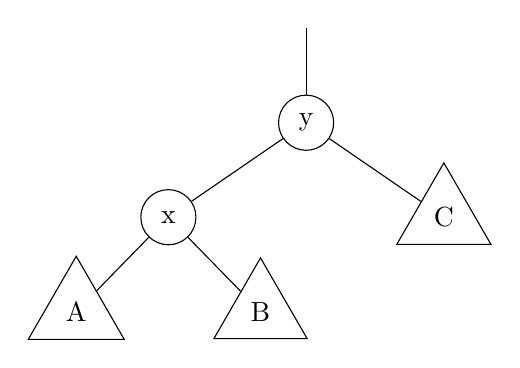
\begin{tikzpicture}[sibling distance=32pt]
\Tree
[ [.y
    [   .x 
        \node[draw,triangle]{A};
        \node[draw,triangle]{B}; ]
    \node[draw,triangle]{C};
] ]
\end{tikzpicture}
\qquad
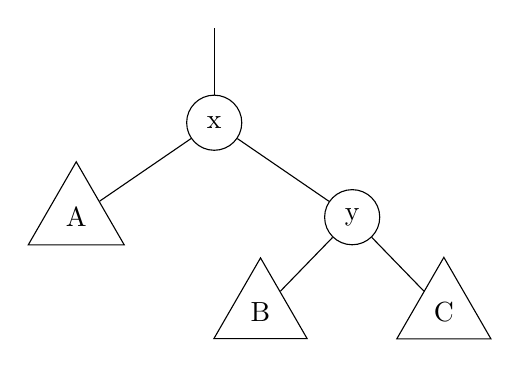
\begin{tikzpicture}[sibling distance=32pt]
\Tree
[ [.x
    \node[draw,triangle]{A};
    [   .y 
        \node[draw,triangle]{B}; 
        \node[draw,triangle]{C}; ]
] ]
\end{tikzpicture}
\end{center}
\caption{Rotate step}
\end{figure}





\section{Original Weak-AVL Tree}

\begin{defn}
A binary tree is said to be {\em ranked binary tree} if all vertices have non-negative integer ranks assigned. External vertices are by convention given rank $-1$. We denote $r(V)$ the rank of vertex $V$.
\end{defn}

\begin{defn}
Vertex $V$ having left child $L$ and right child $R$ (both of which may be external) in ranked binary tree may be said to be either $(a,b)$-vertex or $(b,a)$-vertex if $r(V) - r(L) = a$ and $r(V) - r(R) = b$. $L$ and $R$ are called $a$-child and $b$-child.
\end{defn}

\begin{prop}
Let $S$ be a finite subset of ${(\mathbb{Z} _ +)}^2$ and $T$ a ranked tree with $n$ vertices. If it holds that for every $(i,j)$-vertex in $T$ that $(i,j) \in S$, then the height of $T$ is $\Theta(\log n)$.
\label{thm-rbt-depth}
\end{prop}

\begin{myproof}
Let us denote $m$ the maximum allowed rank difference by $S$.
We prove this by induction on the rank of the root vertex. We establish a lower bound on the number of vertices in a tree with root of rank $r$. 
We suppose that it holds for every lower rank $q$, that the number of vertices in a tree with root of rank $q$ is at least $\exp(qc)$ for some positive constant $c$. 
Then to continue the induction we need the following: $$ 1 + 2\exp((r-m)c) \geq \exp(rc) $$ $$ \log 2 + (r-m)c \geq rc $$ $$ \log 2 \geq cm $$
We see that setting $c$ will be always possible.
The base case of rank zero: The inequality obviously holds for leaves (only possible vertices with rank zero).\\
Then $n \geq \exp(qc)$, if $q$ is the rank of root of $T$. The height of $T$ is in turn at most $ \log(n)/c $. 
The other inclusion applies to all kinds of binary search trees.
\end{myproof}

The theory of ranked trees permits a nice definition of AVL trees\cite{avl}.

\begin{defn}
A ranked tree is said to be {\em AVL tree} if all its every vertex is either $(1,1), (1,2)$ or $(2,1)$  and all leaves are of rank $0$.
\end{defn}

The conditions on rank differences are referred to as rank invariants.

\begin{defn}
A ranked tree is said to be {\em Weak-AVL tree} if all its vertices are either $(1,1), (1,2), (2,1)$ or $(2,2)$ and all leaves are of rank $0$.
\end{defn}

WAVL trees use a relaxation of the balancing rules of AVL trees, this implies that all Weak-AVL trees form a proper subset AVL trees.

From now on, we will ignore symmetric situations. Only one from the pair of $(a,b)$- $(b,a)$- vertices will be considered.

\subsection{Bottom-up rebalancing}

By default WAVL trees use the set of standard set of operations as outlined earlier with rebalancing that is described in this section. A series of steps is taken until the rank invariants are restored.

% Rebalancing consists of checking rank invariant for vertices on the path from the changed vertex back to the root one by one, while performing balancing steps where needed. 

\subsubsection*{Rebalancing after Insert}

Inserting a new leaf $l$ itself may only introduce one type of violation, making the parent of $l$ into a $(0,1)$- or a $(0,2)$-vertex. It will become apparent that the existence of one $(0,1)$- or $(0,2)$-vertex in the tree is the only violation that may happen during this rebalancing. 

Rebalancing after inserts consists of repeatedly checking the rank invariant for vertex $y$. Where $y$ changes during the rebalancing and takes values from the vertices in the BST. Initially $y$ is the parent of the inserted vertex. 

Once the whole subtree of $y$ respects the rank rules, rebalancing proceeds by setting $y$ to be the parent of current $y$. All descendants of $y$ obviously adhere to rank invariant. Either it was not violated by this operation or it has just been amended. 

There are three balancing steps to rectify rank violation at $y$ after insert. (See figures for better illustration.) If rank invariant does not hold for $y$, one of the following steps is chosen, there are symmetric variants for all of these steps. 

\begin{itemize}
	\item \textbf{Promote} If $y$ is a $(0,1)$-vertex, rank of $y$ is increased by 1. This may make the parent of $y$ a $(0,1)$- or $(0,2)$-vertex. Rebalancing thus continues with the parent of $y$ taking role of $y$. (Unless $y$ is the root, then no additional rebalancing is needed.)
	\item \textbf{Rotate} If $y$ is a (0,2)-vertex and the 0-child $x$ is a (1,1)-vertex, we rotate along the edge $xy$. The rank of $y$ is decremented by 1. Rebalancing ends.
	\item \textbf{Double Rotate} If $y$ is a (0,2)-vertex and the 0-child $x$ is a (2,1)-vertex with the 1-child being $w$, we rotate along the edge $xy$ and then along the edge $xw$. Rebalancing ends.
\end{itemize}

One can easily verify that every case is covered by the outlined steps. Most importantly, if rebalancing continues beyond the first vertex, one child of $y$ must be a $(2,1)$-vertex as one of the children must have been promoted and as such it is a $(2,1)$-vertex. This implies existence of an applicable step. 

At the first checked vertex $v$, one of its children has just been inserted. If $v$ was a leaf, promote can be used. If $v$ had one children prior to this insert, it must have rank 1 and insert may be applied. 

\begin{figure}
\begin{center}
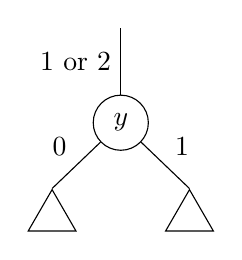
\begin{tikzpicture}[sibling distance=32pt]
\Tree
[ \edge node[auto=right]{1 or 2}; [.$y$
    \edge[tosubtree] node[auto=right] {0};
    \node[draw,triangle]{~};
    \edge[tosubtree] node[auto=left] {1};
    \node[draw,triangle]{~};
] ]
\end{tikzpicture}
\qquad\hspace{20mm}
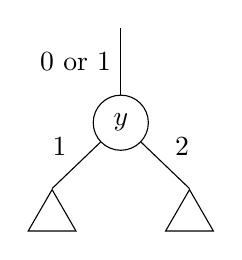
\begin{tikzpicture}[sibling distance=32pt]
\Tree
[ \edge node[auto=right]{0 or 1}; [.$y$
    \edge[tosubtree] node[auto=right] {1};
    \node[draw,triangle]{~};
    \edge[tosubtree] node[auto=left] {2};
    \node[draw,triangle]{~};
] ]
\end{tikzpicture}
\end{center}
{\small The situation displayed on the left depicts the structure prior to the step and the situation on the right after the step. Edges are annotated by rank differences between the endpoint vertices. This convention is followed for depictions of all steps in this section.}
\caption{Promote step}
\end{figure}

\begin{figure}
\begin{center}
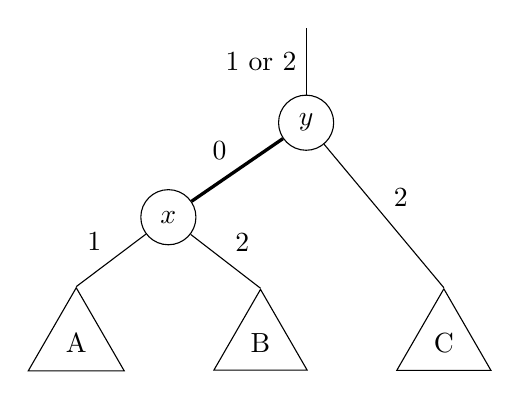
\begin{tikzpicture}[sibling distance=32pt, 
	frontier/.style={distance from root=4cm}]
\Tree
[ \edge node[auto=right]{1 or 2}; [.$y$
    \edge[very thick] node[auto=right] {0};
    [   .$x$ 
        \edge[tosubtree] node[auto=right] {1}; 
        \node[draw,triangle]{A}; 
        \edge[tosubtree] node[auto=left] {2};
        \node[draw,triangle]{B}; ]
    \edge[tosubtree] node[auto=left] {2};
    \node[draw,triangle]{C};
] ]
\end{tikzpicture}
\qquad
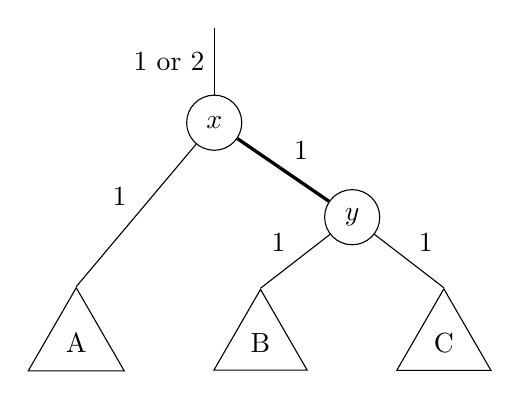
\begin{tikzpicture}[sibling distance=32pt, 
	frontier/.style={distance from root=4cm}]
\Tree
[ \edge node[auto=right]{1 or 2}; [.$x$
    \edge[tosubtree] node[auto=right] {1};
    \node[draw,triangle]{A};
    \edge[very thick] node[auto=left] {1};
    [   .$y$ 
        \edge[tosubtree] node[auto=right] {1}; 
        \node[draw,triangle]{B}; 
        \edge[tosubtree] node[auto=left] {1}; 
        \node[draw,triangle]{C}; ]
] ]
\end{tikzpicture}
\end{center}
\caption{Insert rotation step}
\end{figure}

\begin{figure}.
\begin{center}
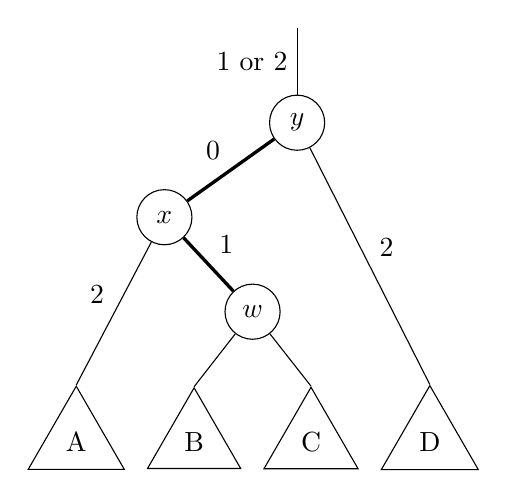
\begin{tikzpicture}[sibling distance=8pt, frontier/.style={distance from root=5.25cm}]
\Tree
[ 
    \edge node[auto=right]{1 or 2}; 
    [
        .$y$
        \edge[very thick] node[auto=right] {0};
        [   
            .$x$ 
            \edge[tosubtree] node[auto=right] {2}; 
            \node[draw,triangle]{A}; 
            \edge[very thick] node[auto=left] {1};
            [
                .$w$
                \edge[tosubtree]; 
                \node[draw,triangle]{B};
                \edge[tosubtree]; 
                \node[draw,triangle]{C}; 
            ]
        ]
        \edge[tosubtree] node[auto=left] {2};
        \node[draw,triangle]{D};
    ] 
]
\end{tikzpicture}
\qquad
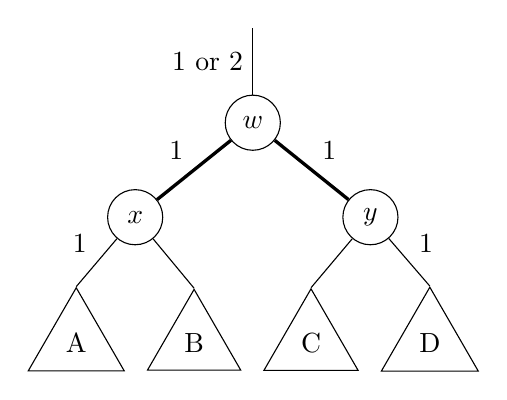
\begin{tikzpicture}[sibling distance=8pt, frontier/.style={distance from root=4cm}]
\Tree
[ \edge node[auto=right]{1 or 2}; [.$w$
    \edge[very thick] node[auto=right] {1};
    [ 
        .$x$
        \edge[tosubtree] node[auto=right] {1};
        \node[draw,triangle]{A};
        \edge[tosubtree];
        \node[draw,triangle]{B};
    ]
    \edge[very thick] node[auto=left] {1};
    [   .$y$ 
    	\edge[tosubtree];
        \node[draw,triangle]{C}; 
        \edge[tosubtree] node[auto=left] {1}; 
        \node[draw,triangle]{D}; ]
] ]
\end{tikzpicture}
\end{center}
\caption{Insert double rotation step}
\end{figure}

\subsubsection*{Rebalancing after Delete}

This process is analogous to reblancing after insert in many ways. Deleting a leaf may cause its former parent to become either a $(3,1)$-vertex, a $(3,2)$-vertex, a $(2,2)$-vertex that is a leaf, or a $(2,1)$-vertex. This is easily seen from examining all possibilities. 

Starting from the parent of the deleted vertex, going towards the root, the rank invariant is checked for every vertex $y$ on that path.  During the rebalancing only one vertex may violate the rank invariant at a time and if so, it must either $(3,1)$ or $(3,2)$, (with the exception of the initial $(2,2)$-leaf).

There are four different balancing steps, one of which is applied if the rank invariant does not hold at $y$. (Again, these are illustrated in figures.)
\begin{itemize}
	\item \textbf{Demote} If $y$ is a $(3,2)$-vertex or a $(2,2)$-leaf, the rank of $y$ is decremented by 1 and rebalancing continues with the parent of $y$ taking the role of $y$. (If $y$ is the root, rebalancing ends.)
	\item \textbf{Demote of the Second Kind} If $y$ is a $(3,1)$-vertex and its 1-child is a $(2,2)$-vertex, the rank of $y$ and its 1-child is decremented by 1 and rebalancing continues with the parent of $y$ taking the role of $y$. (If $y$ is the root, rebalancing ends.)
	\item \textbf{Rotate} If $y$ is a $(3,1)$-vertex, the 1-child $x$ is the right child and its right child is 1-child, we rotate along $xy$, decrementing rank of $y$ by 1 and incrementing the rank of $x$. Rebalancing ends. Of course, in the symmetric case when the 1-child is the left child, symmetric changes must be applied.
	\item \textbf{Double Rotate} If $y$ is a $(3,1)$-vertex, the 1-child $x$ is the right child and a $(2,1)$-vertex and also the 2-child $w$ of $x$ is its left child, we rotate along $xy$ and then along $wy$, decrementing rank of $y$ by 2, of $x$ by 1 and incrementing the rank of $w$ by 2. Rebalancing ends. Of course, in the symmetric case when the 1-child is the left child, symmetric changes must be applied.
\end{itemize}

\begin{figure}
	\begin{center}
		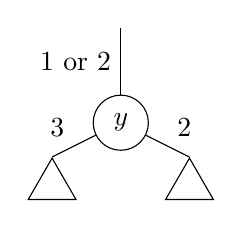
\begin{tikzpicture}[sibling distance=32pt, frontier/.style={distance from root=2cm}]
		\Tree
		[ \edge node[auto=right]{1 or 2}; [.$y$
		\edge[tosubtree] node[auto=right] {3};
		\node[draw,triangle]{~};
		\edge[tosubtree] node[auto=left] {2};
		\node[draw,triangle]{~};
		] ]
		\end{tikzpicture}
		\qquad
		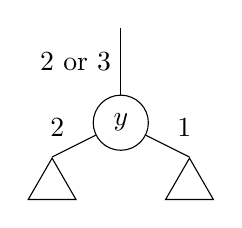
\begin{tikzpicture}[sibling distance=32pt, frontier/.style={distance from root=2cm}]
		\Tree
		[ \edge node[auto=right]{2 or 3}; [.$y$
		\edge[tosubtree] node[auto=right] {2};
		\node[draw,triangle]{~};
		\edge[tosubtree] node[auto=left] {1};
		\node[draw,triangle]{~};
		] ]
		\end{tikzpicture}
	\end{center}
	\caption{Demote step of the first kind}
\end{figure}


\begin{figure}
	\begin{center}
		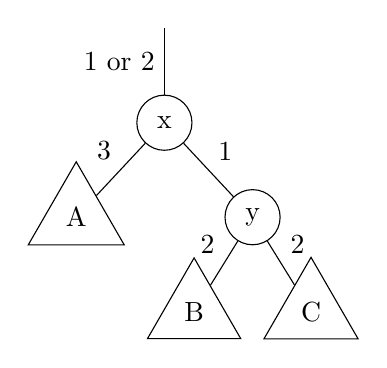
\begin{tikzpicture}[sibling distance=8pt]
		\Tree[ 
		\edge node[auto=right] {1 or 2};
		[   
		.x 
		\edge node[auto=right] {3}; 
		\node[draw,triangle]{A}; 
		\edge node[auto=left] {1};
		[
		.y
		\edge node[auto=right] {2};
		\node[draw,triangle]{B};
		\edge node[auto=left] {2};
		\node[draw,triangle]{C}; 
		] ] ]
		\end{tikzpicture}
		\qquad
		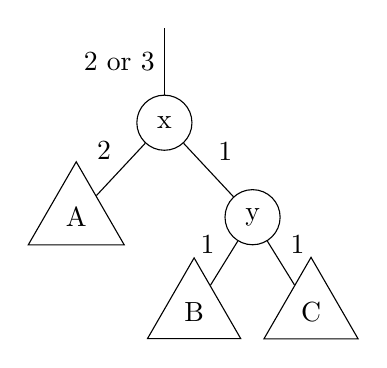
\begin{tikzpicture}[sibling distance=8pt]
		\Tree[ 
		\edge node[auto=right] {2 or 3};
		[   
		.x 
		\edge node[auto=right] {2}; 
		\node[draw,triangle]{A}; 
		\edge node[auto=left] {1};
		[
		.y
		\edge node[auto=right] {1};
		\node[draw,triangle]{B};
		\edge node[auto=left] {1};
		\node[draw,triangle]{C}; 
		] ] ]
		\end{tikzpicture}
	\end{center}
	\caption{Demote of the second kind step}
\end{figure}


\begin{figure}
\begin{center}
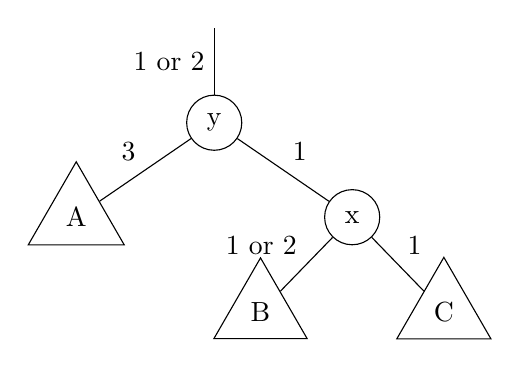
\begin{tikzpicture}[sibling distance=32pt]
\Tree
[ \edge node[auto=right]{1 or 2}; [.y
    \edge node[auto=right] {3};
    \node[draw,triangle]{A};
    \edge node[auto=left] {1};
    [   .x 
        \edge node[auto=right] {1 or 2}; 
        \node[draw,triangle]{B}; 
        \edge node[auto=left] {1};
        \node[draw,triangle]{C}; ]
] ]
\end{tikzpicture}
\qquad
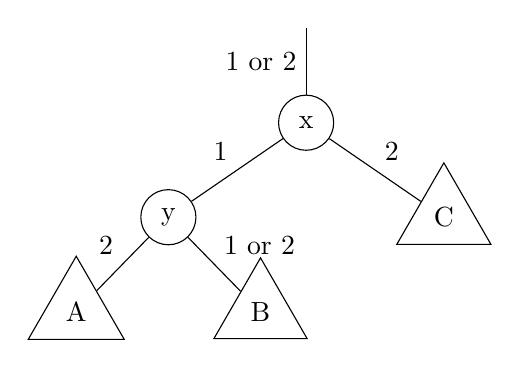
\begin{tikzpicture}[sibling distance=32pt]
\Tree
[ \edge node[auto=right]{1 or 2}; [.x
    \edge node[auto=right] {1};
    [ .y 
        \edge node[auto=right] {2}; 
        \node[draw,triangle]{A}; 
        \edge node[auto=left] {1 or 2}; 
        \node[draw,triangle]{B}; ]
    \edge node[auto=left] {2};
    \node[draw,triangle]{C};
] ]
\end{tikzpicture}
\end{center}
\caption{Delete rotation step}
\end{figure}

\begin{figure}
\begin{center}
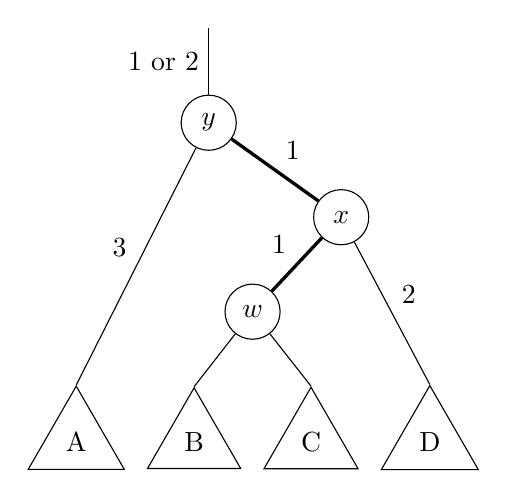
\begin{tikzpicture}[sibling distance=8pt, frontier/.style={distance from root=5.25cm}]
\Tree
[ 
    \edge node[auto=right]{1 or 2}; 
    [
        .$y$
        \edge[tosubtree] node[auto=right] {3};
        \node[draw,triangle]{A};
        \edge[very thick] node[auto=left] {1};
        [   
            .$x$ 
            \edge[very thick] node[auto=right] {1};
            [
                .$w$
                \edge[tosubtree];
                \node[draw,triangle]{B};
                \edge[tosubtree];
                \node[draw,triangle]{C}; 
            ]
            \edge[tosubtree] node[auto=left] {2}; 
            \node[draw,triangle]{D}; 
        ]
    ] 
]
\end{tikzpicture}
\qquad
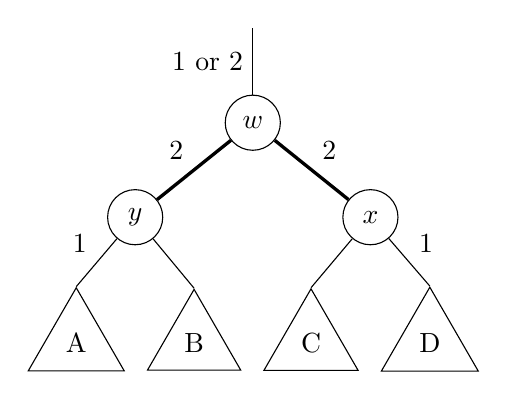
\begin{tikzpicture}[sibling distance=8pt, frontier/.style={distance from root=4cm}]
\Tree
[ \edge node[auto=right]{1 or 2}; [.$w$
    \edge[very thick] node[auto=right] {2};
    [ 
        .$y$
        \edge[tosubtree] node[auto=right] {1};
        \node[draw,triangle]{A};
        \edge[tosubtree];
        \node[draw,triangle]{B};
    ]
    \edge[very thick] node[auto=left] {2};
    [   .$x$ 
    	\edge[tosubtree];
        \node[draw,triangle]{C}; 
        \edge[tosubtree] node[auto=left] {1}; 
        \node[draw,triangle]{D}; ]
] ]
\end{tikzpicture}
\end{center}
\caption{Delete double rotation step}
\end{figure}

With the rebalancing processes described, we get the following as a corollary of theorem \ref{thm-rbt-depth}.

\begin{prop}
Insertion and deletion on a Weak AVL tree $T$ have time complexity $\Theta(\log n)$ and require at most one rotation. Here $n$ denotes the number of vertices in $T$.
\end{prop}

It is time to list additional properties of WAVL trees, which will be useful later. The proofs are beyond the scope of this thesis and can be found in an article by Haeupler, Sen, and Tarjan \cite{rank-balanced-trees}. These results are obtained by cleverly defining a potential function on vertices of the BST.

\begin{thm}
In a WAVL tree with bottom-up rebalancing, there are \bigO{d} demote steps over all operations, where $d$ denotes the total number of deletions. (With the tree initially empty.)
\end{thm}

\begin{thm}
In a WAVL tree with bottom-up rebalancing, there are \bigO{m} promote steps over all operations, where $m$ denoted the total number of insertions. (With the tree initially empty.)
\end{thm}

WAVL trees have good properties when we consider the amortized number of promote, demote, or rotate steps -- all average to a constant. The number of rotations is constant even in the worst case. Unfortunately, we will need constant number of modifications per update even in the worst-case.

\subsection{Top-down rebalancing}

There is an alternative set of procedures for performing insert and delete in WAVL tree. Changes are performed during descent from the root while searching for the key in question. No return to the root ensues.

For insert, we know that problematic vertices that cause promote to be passed upwards are $(0,1)$. Such vertices come to exist from $(1,1)$-vertices by promoting one of their children. Passing through a vertex other than $(1,1)$ ensures that rebalancing will not proceed through that vertex upwards. We thus only need to worry about long chains of $(1,1)$-vertices when descending during the find phase of insert. When we traverse the tree down from the root during the find phase, these must removed.

Top-down rebalancing utilizes \emph{forced reset} to remove these long chains of $(1,1)$-vertices. Forced reset is triggered by passing through the $k$-th $(1,1)$-vertex (denoted $d$) in a row during the find phase of insert. The last passed node that is not $(1,1)$ (or root) is called \textit{safe node}. We know that promoting $d$ might require rebalancing to be performed starting at $d$ to restore rank rules. We know however that this rebalancing will end at the safe node, taking \bigO{1} operations.
With forced-reset prevents returning arbitrarily close to the root during rebalancing after the insert is performed.

Similarly with delete, in which case problematic nodes are $(2,2)$ and $(2,1)$ with the 1-child being $(2,2)$. The remaining nodes are safe. Forced-reset triggers demote after passing through $l$ non-safe nodes. (Subsequent rebalancing ends after \bigO{1} steps.)

As the next theorem claims, we can preserve the upper bound on rebalancing steps, the number of rotations during one operation unfortunately can be as high as \bigO{\log n}.

\begin{thm}
Setting $k=5$ and $l=3$, top-down rebalancing takes \bigO{m+d} steps where $m$ denotes the number of inserts and $d$ the number of deletes.
\end{thm}

We also get another pleasant property with top-down rebalancing.

\begin{defn}
Insert and delete operation is said to be of rank $r$ if the highest rank of a vertex where rotation or rank change takes place is $r$.
\end{defn}

\begin{thm}
With $k=5$ and $l=3$, there exists a positive constant $c > 1$ such that top-down rebalancing takes \bigO{mc^{-r}} rebalancing steps of order $r$ where $m$ denotes the number of total inserts.
\end{thm}

\section{Weight-balanced tree}

In our algorithm for persistent binary tree, we will also need weight-balanced (originally BB[$\alpha$]) trees. Here we describe their properties.

Weight-balanced trees form a class of binary search trees. The strategy of maintaining balance in weigh-balanced trees uses a different approach from that of rank-balanced trees.

A vertex of a weight-balanced tree has these entries stored (in addition to key and value): {\em size} of subtree rooted at that vertex and pointers to {\em left} and {\em right} child. By definition the size of external vertex is 0. {\em Weight} of a vertex is then defined as size + 1.

\begin{defn}
Let $\alpha \in (0,1/2)$ be constant. We call a binary search T an {\em $\alpha$-weight-balanced tree} if it holds for every vertex $v$ of T that $weight(left(v)) \geq \alpha \cdot weight(v)$ \& $weight(right(v)) \geq \alpha \cdot weight(v) $.
\end{defn}

\begin{prop}
Let $\alpha \in (0,1/2)$ be constant. Every $\alpha$-weight-balanced tree $T$ with $n$ vertices has depth $\Theta(\log n)$. 
\end{prop}

\begin{myproof}
Let us consider an inner vertex of size $s$ with children of sizes $s_l$ and $s_r$. Then from the definition of weight-balanced trees:

$$s_l + 1 \geq \alpha (s_r+1)$$
$$ s = s_l + s_r + 1 $$
$$ s \geq \alpha (s_r+1) + s_r $$
$$ s \geq (1+\alpha)s_r $$

Which implies that size of parent is at least a constant factor greater than of each of its children.
\end{myproof}

Now we turn to the algorithm for insertion. (Deletion is similar and will not be discussed as we do not need it in this thesis). As usual we determine the place of insertion and insert the vertex. Next we update sizes of all vertices on the path toward the root. This can break balance of some vertices on this path, with $v$ being closest to the root. If $v$ exists, the entire subtree rooted at $v$ is reconstructed into a perfectly balanced binary tree.

It can be proven that the asymptotic cost of this insert is logarithmic.

\begin{prop}
Any $n$ consecutive operations performed on initially empty weight-balance tree have total complexity $\mathcal{O}(n \log n)$. 
\end{prop}

\section{Alternative WAVL Tree Balancing Algorithm}

For our purposes standard algorithm for working with WAVL trees cannot be used. It is guaranteed that no more than one rotation occurs during insert or delete. Nonetheless, the number of rank changes can be up to $O(\log n)$. 

Fortunately, the algorithm can be modified in such a way that no operation requires more than $O(1)$ changes. It will come with the price of roughly four times as many rules for balancing. Given that WAVL trees compared to AVL trees already have noticeably more complicated implemntation, this makes the structure ill suited for other usege. 

The problems in WAVL trees arose from promote and demote operations which can propagate from the inserted (respectively deleted) vertex all the way to the root. We will call the sequence of vertices that had their ranks increased by promote during one insertion a {\em promotion path}. Similarly, all vertices demoted during one deletion will be refered to as a {\em demotion path}. Our modifications handles all changes along such paths as one modification. Only one such path is created using the standard rules and up to one other can be split during an operation. With the required rotation, these are the only changes performed by our alternative algorithm.

%Is it not two extra paths?

An extra field is added to each vertex if it is the top of a {\em modifying path}, i.e. promotion or demotion path. It indicated promotion or demotion and points to the bottom vertex of the path.

A vertex can be a part of at most one modifying path at any time, this will become apparent from the procedures for insert and delete. When descending down the tree, it is easy to determine where we leave the modifying path. When we compare the value of a vertex to searched key, we also compare to the end of modifying path and if the comarison outcomes differ, we leave the path at this vertex. 

Rank of vertices that belong to a modifying path can be inferred rather easily. If we know that a promotion path continues here, the value should be increased by one. If a demotion path continues through, the type of demotion is determined from the rank of the child not on the path. The only tricky part is the second case of demote where rank of vertices not on the path is decreased, although this poses a mere inconvenience for implementation, not a fundamental problem.

\subsection{Find, Predecessor \& Successor}

Since promote and demote steps do not change the structure of the tree (they only change the ranks), all searching operations remain identical.

\subsection{Insert}

Inserts starts from the root of the tree. We use a stack to keep the list of vertices visited, we add those with calculated actual ranks and with pointers to start and end of the modifying path they are on, where applicable.

When the insertion is performed, we start ascension back to the root. During this stage we use the stack with paths to be aware of true ranks. If there are no vertices violation the rank invariants, the insertion process ends. Otherwise we will use one of the rules prescribed the standard algorithm, but we also have to take special care with ends of modifying paths. The paths are either shortened or destroyed when their length becomes one -- we simply adjust the rank of the last vertex on such path. Below is the list of all cases that can arise based on the type of vertex that is being processed.

\textbf{Current vertex is not on any modifying path.} In this case, the rank invariant is checked. 

\begin{itemize}

\item If rank invariant holds, it remains to end newly created nodifying path at its last vertex. Should it have just 1 or 2 vertices, their ranks are adjusted immediately. If the invariant fails however, one of the three steps for fixing this must be identified. Rebalancing ends.

\item If promote is necessary, beginning of promotion path is marked. If there is promotion path open already, it is extended by one vertex.

\item If simple rotation is necessary, it is performed. If there a path open its top must be marked, unless it were at most 2 vertices long, in that case, those vertices should have thier ranks adjusted. If the other child of this vertex is on a path, it is the top of that path, such path is then shoretened or destroyed. Rebalancing stage ends by this step.

\item If double rotation is necessary, it is also performed. Similarly, paths are shortened. Rebalancing ends.

\end{itemize}

\textbf{Current vertex is on a promotion path.} We know this was a (1,2) vertex before changes done in this insertion. We proceed by checking rank inveriant. 

\begin{itemize}

\item If rank invariant holds, it remains to end newly created nodifying path at its last vertex just as in the previous cases. If this vertex ceased to be (1,2) vertex, it will have its rank increased and will be removed from this path it is on. Rebalancing ends.

\item We know that promote will not be needed, one of the children of this vertex might have its rank increases. It is only possible for (0,1) vertex to be promoted, this vertex must be either (0,2), (1,1) or (1,2) though.

\item If simple rotation is necessary, it is performed. Again paths are handled, this vertex is removed from the path it is on. Rebalancing ends in this step.

\item If double rotation is necessary, it is also performed. Similarly, paths are shortened. Rebalancing ends.

\end{itemize}

\textbf{Current vertex is on a demotion path.} We know this was a (1,2) vertex before changes done in this insertion. We proceed by checking rank invariant. 

\begin{itemize}

\item If rank invariant holds, it remains to end newly created nodifying path at its last vertex just as in the previous cases. If this vertex ceased to be (1,2) vertex, it will have its rank decreased and will be removed from this path it is on. Rebalancing ends.

\item We know that promote will not be needed, one of the children of this vertex might have its rank increases. It is only possible for (0,1) vertex to be promoted, this vertex must be either (0,2), (1,1) or (1,2) though.

\item If simple rotation is necessary, it is performed. Other paths are handled, this vertex is removed from the path it is on. Rebalancing ends in this step.

\item If double rotation is necessary, it is also performed. Similarly, paths are shortened. Rebalancing ends.

\end{itemize}

\textbf{Current vertex has its rank externally decreased by its parent on a demotion path.} We know this was a (1,1) vertex before changes done in this insertion. We proceed by checking rank invariant. 

\begin{itemize}

\item If rank invariant holds, this vertex is still (1,1) vertex. No path operation are needed. Rebalancing ends.

\item If promote is required, rotation will ensue at parent of this vertex. This both these vertices are removed from excluded from all paths and rotation at parent is executed. Again, paths are shortened where needed. Rebalancing ends.

\item Simple rotation will not be needed.

\item Double rotation will not be needed.

\end{itemize}

As a side-node we mention that a vertex on a demotion path that decreases rank of its one child be be excluded from this path even if that child stops being a (1,1) vertex.

\subsection{Delete}

The process is very similar to insert. First, if the vertex cannot be deleted directly, the vertex bearing the next lower/higher key must be identified and the keys \& values exchanged. Then search for the key about to be deleted (which is now in a leaf) starts from the root. In this stage he stack of vertices is maintained just as in insert step. 

Once a node is deleted, balancing steps are taken starting from the parent of deleted node, continuing to root. Standard deletion rules are used. Below is the list of all cases that can arise based on the type of vertex that is being processed.

\textbf{Current vertex is not on any modifying path.} In this case, the rank invariant is checked. 

\begin{itemize}

\item If rank invariant holds, it remains to end newly created nodifying path at its last vertex. Should it have just 1 or 2 vertices, their ranks are adjusted immediately. Rebalancing ends.

\item If demote is necessary, beginning of promotion path is marked. If there is a demotion path open already, it is extended by one vertex. We also note that if adding this vertex to demotion path implicitly decreases the rank of one of its children, the child is not on any modifying path. Only (1,2) vertices can be.

\item If simple rotation is necessary, it is performed. If there a path open its top must be marked, unless it were at most 2 vertices long, in that case, those vertices should have thier ranks adjusted. If the other child of this vertex is on a path, it is the top of that path, such path is then shoretened or destroyed. Rebalancing stage ends by this step.

\item If double rotation is necessary, it is also performed. Similarly, paths are shortened. Rebalancing ends.

\end{itemize}

\textbf{Current vertex is on a promotion path.} We know this was a (1,2) vertex before changes done in this insertion. We proceed by checking rank invariant. 

\begin{itemize}

\item If rank invariant holds, it remains to end newly created nodifying path at its last vertex just as in the previous cases. If this vertex ceased to be (1,2) vertex, it will have its rank increased and will be removed from this path it is on. Rebalancing ends.

\item If demote is needed, it is easy to verify, that this vertex is the bottom of its promotion path, the path is simply shortened or destroyed and rebalancing ends. One child can potentially have its rank decreased. Open demotion path is closed with the other child as top or destroyed if too short.

\item If simple rotation is necessary, it is performed. Again paths are handled, this vertex is removed from the path it is on. Rebalancing ends in this step.

\item If double rotation is necessary, it is also performed. Similarly, paths are shortened. Rebalancing ends.

\end{itemize}

\textbf{Current vertex is on a demotion path.} We know this was a (1,2) vertex before changes done in this insertion. We proceed by checking rank invariant. 

\begin{itemize}

\item If rank invariant holds, it remains to end newly created modifying path at its last vertex just as in the previous cases. If this vertex ceased to be (1,2) vertex, it will have its rank decreased and will be removed from this path it is on. Rebalancing ends.

\item It is easy to see that vertices must be removed from a demotion prior to any subsequent demotions. Demotion will not be needed.

\item If simple rotation is necessary, it is performed. Other paths are handled, this vertex is removed from the path it is on. Rebalancing ends in this step.

\item If double rotation is necessary, it is also performed. Similarly, paths are shortened. Rebalancing ends.

\end{itemize}

\textbf{Current vertex has its rank externally decreased by its parent on a demotion path.} We know this was a (1,1) vertex before changes done in this insertion. We proceed by checking rank invariant. 

\begin{itemize}

\item If rank invariant holds but this vertex has become a (1,2) vertex. Parent must be removed from demotion path and rank changes put into effect. Rebalancing ends.

\item Demote will not be required this vertex can only be (1,1) or (1,2).

\item Simple rotation will not be needed.

\item Double rotation will not be needed.

\end{itemize}


\chapter{Persistence}

In this chapter we finally arrive to our main interest. First of all we introduce the hierarchy of data structures with respect to persistence.

\begin{itemize}
\item {\bfseries Ephemeral data structures} are the most widespread. 
Past states are destroyed by "destructive" updates and irretrievably lost.
\item {\bfseries Semi-persistent data structures} (sometimes partially persistent) 
still support modifying operations only on the most recent version. 
Updates produce a new version of the structure. 
Historical versions form a linear order. 
Past states can be reconstructed efficiently for reading.
\item {\bfseries (Fully-)persistent data structures} directly extend their semi-persistent counterparts. 
An update can be done on any version of the structure, resulting in a rooted tree of versions. 
An update corresponds to adding a new child vertex to an existing vertex in the tree.
\item {\bfseries Functional data structures} permit no changes to data once written. 
Naturally, persistence is guaranteed under such an assumption, 
as all versions appear as if just created by the last update.
This enforced immutability completely freezes past version in time.
This concept is intrinsic to functional languages such as Haskell, 
but proves to be useful even in imperative programming. 
Multi-threading is easier when there is confidence that existing objects will not be modified.
\end{itemize}.

This division is by no means universally adopted, but provides an interesting perspective regardless.

With a persistent data structure, we essentially want to have one data structure for every existing version. Insert and delete return a new version handle instead of making changes to the existing version. Obviously, copying the data structure every time is one option how to achieve this, albeit not a great one. To prevent using extra memory and increased time complexity of operations however, more intricate methods must be employed.

Going beyond this hierarchy, if fully-persistent data structure also supports merging or melding two different versions, it is said to be \emph{confluently persistent}. Confluently persistent data structures are the subject of studies for example by Driscoll, Sleator, and Tarjan\cite{confluently-persistent-a} or Fiats and Kaplan\cite{confluently-persistent-b}. We will not investigate confluent persistence in this thesis further.

\section{Persistence through Path-Copying}

Let us open with a few simple constructions first. Binary search tree can be converted into a fully-persistent one rather easily.
The straight-forward approach is called path-copying. It is based on the observation that most of the tree does not change during an update.

When a new version of the tree should by created by delete or insert, new copies are allocated only for vertices that are changed by the operation and their ancestors. 
This typically means that only path from the inserted/deleted vertex to the root is newly allocated, plus constant number of other vertices. 
The new vertices carry pointers to the old vertices where subtree rooted at such a vertex is not modified in any way.
Here we tacitly assume that only pointers to children are stored. Updating root in a tree with pointers to parents would involve creating new instances for all nodes in the tree.

With reasonable variants of binary search trees, achieved time complexity in a tree with $n$ vertices is $\Theta(\log n)$ per operation and $\Theta(\log n)$ memory for insert/delete.

The downside of this method is the increased space complexity. There is no apparent construction that would not increase memory complexity by copying the paths.

\section{Multiple versions in one vertex}

To limit memory consumption we may rather choose to let vertices carry their properties for all versions. This in reality means that we must store a collection of changes together with versions when those changes happened. This makes a vertex a kind of dictionary with keys being versions and values the descriptions of changes.

When semi-persistence is sufficient, upon arriving at a vertex asking for the state in version $A$, we do the following: We must go through the collection of changes to figure out what the state in version $A$ should be. 
We start with the default values and apply all changes that happened earlier than $A$ in chronological order overwriting if there are multiple changes for the same field or pointer. 
This process yields the correct state of the vertex for version $A$. 

In fact, it might be easier to just copy all of the other fields the vertex possesses as well if one of them changes.
One change will therefore hold new values for all fields and pointers of the vertex. 

For full-persistence we also need to resolve the issue of how to effectively determining which changes should be applied. 
It will be addressed later through introduction of total ordering of all versions.

Looking at the memory consumption, it appears clear that the amount consumed stems from the total number of changes done by the balancing algorithm across all operations.

What remains to solve though is to choose the right kind of collection for versions of changes for one vertex. Surely using linked lists or arrays will inevitably lead to unsatisfactorily inefficient processing of applicable changes. Unfortunately as it turns out, even other data structures will let us down here.

With this approach, we can reach space complexity that is linear with the total number of changes in the tree. On the other hand execution time will be hurt. We can reach the following amortized complexity depending on the chosen data structure:

\begin{tabular}{ll}
Linked list & \bigO{n \log n} \\
Binary search tree & \bigO{\log^2 n} \\
Q-fast trie \cite{q-fast-trie} & \bigO{\log ^{3/2} n}, semi-persistence only \\
Y-fast trie \cite{y-fast-trie} & \bigO{\log n \cdot \log \log n}, semi-persistence only, on average

\end{tabular}

\begin{figure}
	\begin{center}
		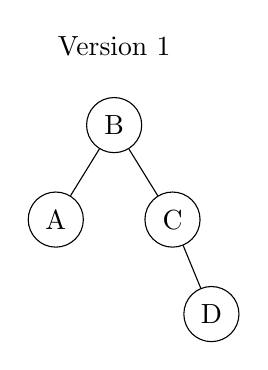
\begin{tikzpicture}[sibling distance=8pt]
		\Tree[
		.B A [ .C \edge[blank]; \node[blank]{}; D ]
		]
		\node at (0,1) {Version 1};
		\end{tikzpicture}
		\qquad\hspace{40mm}
		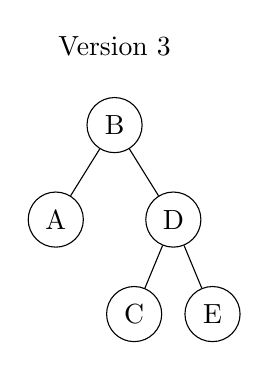
\begin{tikzpicture}[sibling distance=8pt]
		\Tree[
		.B A [ .D C E ]
		]
		\node at (0,1) {Version 3};
		\end{tikzpicture}
	\end{center}
\raggedcolumns
\begin{multicols}{2}
\centering
\footnotesize
\begin{vdTable}{Vertex}
	Version & Left & Right   & Key & Value
\end{vdTable}
\begin{vdTable}{A}
	1 & $\Lambda$ & $\Lambda$ & 10 & 5 \\
	2 & $\Lambda$ & $\Lambda$ & 10 & 6
\end{vdTable}
\begin{vdTable}{B}
	1 & A & C & 20 & 15 \\
	3 & A & D & 20 & 15
\end{vdTable}
\begin{vdTable}{C}
	1 & $\Lambda$ & D & 30 & 27 \\
	3 & $\Lambda$ & $\Lambda$ & 30 & 27
\end{vdTable}
\begin{vdTable}{D}
	1 & $\Lambda$ & $\Lambda$ & 40 & 39 \\
	3 & C & E & 40 & 39
\end{vdTable}
\begin{vdTable}{E}
	3 & $\Lambda$ & $\Lambda$ & 50 & 99
\end{vdTable}\\
\end{multicols}

Tree is shown for version 1 (left) and 3 (right). Internal collections for each vertex are displayed. Operation that created version 2 changed value of key 10. Operation that created version 3 inserted vertex E and triggered a rotation. Faithful to The Art of Computer Programming, $\Lambda$ represents a null pointer.
\caption{A tree with dictionaries in vertices} 

\end{figure}

\section{Fat Vertices}

Following up on the idea of multiple versions in one vertex, fat vertices were devised. 
We will explain this technique only for semi-persistence first. 
Full persistence requires the use of a few extra tricks and establishing an ordering on the versions.

A fat vertex stores a dictionary of standard vertices indexed by versions. 
We call values of this dictionary slots. 
The maximum size of this dictionary is set to a constant which is to be determined later. 
Temporarily, we will allow the capacity of fat vertex to be exceeded. 
This will have to be fixed however, before the ongoing operation finishes.
By placing a restriction on the size we may circumvent the increased complexity of search within one vertex.
Instead of copying the vertex, we simply add new slot into the dictionary. 
Provided the maximum has not been exceeded yet, this insertion of a slot stops the propagation of changes toward the root. 
The Reader should recall that this was the major weakness of path-copying.
Because of the limit on size of this dictionary, it may be implemented simply as a linked list.

Contents of one slot are a version handle, all pointers a vertex would have, then inverse pointers to fat vertices that have slots pointing to this fat vertex for this version and some fields, notably key and value as a bare minimum.
Not all fields need to be versioned. 
For example balancing information may be stored only for the latest version, i.e. in red-black trees color is only used for balancing and is thus not needed to be persisted for old versions. 
(Until full-persistence comes into play.)

One vertex in the original binary search then corresponds to a doubly-linked list of fat vertices.
When the vertex changes, new state of the vertex is written into a slot of the last fat vertex in the list. 
As all slots become occupied in the last fat vertex and it needs to be modified, new vertex is allocated.

Modifications of a single vertex during one operation are all written to single slot, there is no need for using more slots.

When a new fat vertex $x$ is allocated, one of its slots is immediately taken. 
Pointers must be updated in other fat vertices that pointed to the fat vertex preceding $x$ in the list. 
This is done either by inserting new slot into them (copying all values from the latest slot and replacing pointers to the predecessor by pointers to $x$). 
Or by directly updating the pointers if the right version is already present. 

Recursive allocations may be triggered, which is not a problem if there is only a small amount of them. 
This is ensured by setting the size of fat vertices suitably. 
The order in which these allocations are executed can be arbitrary.
We can place an upper bound on the number of newly allocated fat vertices -- total number of vertices in the tree (including deleted vertices). 
At most one new slot is occupied for every vertex in the tree.

To take advantage of fat vertices, we need the balancing algorithm to limit the number of vertices that change in one operation. 
This was the goal of modified WAVL-balancing algorithm all along. 
Furthermore, we need a limit on the number of pointers that can target one vertex at one time.

\begin{prop}
Suppose any binary search tree balancing algorithm satisfying the following properties:
\begin{itemize}
\item 
There is a constant $k$ such that for any $n$ successive operations on initially empty tree, the number of vertex changes made to the tree is at most $kn$. 
\item 
There is a constant bound on the number of pointers to any one vertex at any time.
\end{itemize}
Then this algorithm with the addition of fat vertices for semi-persistence, consumes \bigO{n} space for the entire history of $n$ operations starting from an empty tree.
\end{prop}

\begin{myproof}
We denote the number of pointer fields per vertex as $p$ and maximum number of vertices pointing to one vertex at a time as $x$. We then define the number of slots in fat vertex as $s = p + x + 1$. (Higher value is also possible)\\
We define the potential of the structure as the total number of occupied slots in all fat vertices that are the last in their doubly-linked list. (Thus initially zero.) Allocation of a new fat vertex will cost one unit of energy. This cost can be charged from the potential or the operation. We will show that the operation needs to be charged only a constant amount of energy per one vertex modification by the original algorithm (to compensate increase in potential or pay for allocations), from which the proposition follows.\\
For insert, a new vertex is created (which increases potential by a constant). During rebalancing of the tree, $r$ vertices are to be modified. Let us consider this sequence of modifications one by one. We send one floating unit of energy to each of the $r$ vertices.\\
If a modification of $v$ is second or later modification of $v$ during this operation, changes are simply written to the slot for this version.\\
Otherwise, number of used slots is checked. If there is one or more empty available, new slot is used, taking default values of fields from preceding slot. This increases potential by one, which is covered by the floating unit of energy.\\
If no slots are available, new fat vertex $v'$ is allocated and one of its slots is used. This step triggers a decrease in the potential by $p+x$. The floating unit of energy is used to pay for allocation of the new vertex. Next, fat vertices to corresponding current version interval of vertices having pointers to $v$ need to have this reflected. Additionally inverse pointers to $v'$ need to be set. These are at most $p+x$ changes to other vertices that may use their new empty slots. The decrease in potential is used to send one unit of energy to every such vertex that need an update. Changes are executed recursively and will not require extra energy to be charged on this modification.
\end{myproof}

Regarding the time complexity, searching the correct slot in a fat vertex produces only constant overhead. Realizing that every operation can be charged on a memory allocation of a fat vertex such that there is a constant $c$ depending only on the balancing algorithm such that for every allocated fat vertex the number of operations charged on it is at most $c$.

\begin{obs}
Assuming the conditions from the previous proposition, the cost to write changes into fat vertices is amortized to \bigO{1} per operation.
\end{obs}

We see that WAVL trees can be used for semi-persistence even in their original form, along with many other binary search trees. Time complexity of operations with the tree depends on the original balancing algorithm used. With WAVL trees we get \bigO{\log n} per operation from the original algorithm in addition to the amortized \bigO{1}. Here $n$ is the size of the tree in the version that is queried.

In fact, for semi-persistence fat vertices may be defined differently. It suffices that only values of changed fields and pointers are written into slots. Thus each fat vertex carries a set of default values for every field and pointer, these values are used if not overridden by a slot. This approach may lead to lower memory consumption and is not directly compatible with the approach to full persistence described later.

\begin{figure}
\begin{center}
	\ttfamily
	\begin{tabular}{cccccc}
		Rank  & Previous &  Next   &      & &          \\ \hline
		Left1 &  Right1  & Parent1 & Key1 & Value1 &  Version1 \\ \hline
		Left2 &  Right2  & Parent2 & Key2 & Value2 & Version2 \\ \hline
		Left3 &  Right3  & Parent3 & Key3 & Value3 & Version3 \\ \hline
		Left4 &  Right4  & Parent4 & Key4 & Value4 & Version4 \\ \hline
		Left5 &  Right5  & Parent5 & Key5 & Value5 & Version5 \\ \hline
		Left6 &  Right6  & Parent6 & Key6 & Value6 & Version6 \\ \hline
	\end{tabular}
\end{center}
Rank of WAVL trees is not used for navigation only for balancing the tree, it need not be maintained for older versions.
\caption{Layout for WAVL semi-persistent tree fat vertex}
\end{figure}

\section{Parallel Semi-Persistence with WAVL Trees}

Recall that insertion and deletion in a WAVL tree can be also carried out top-down.
By preemptively performing rotations, promotes and demotes when descending, we can make sure that large number of changes of vertices with high ranks will not be needed. This means that as insert or delete will descend down the tree towards the leaves processing vertices along some vertical path, it will hold locks for vertices in at most constant distance from the vertex that the operation is currently processing.

Also recall that there are at most \bigO{1} modifications of the structure per update (amortized), albeit the constant proves to be rather high. These facts lay a solid foundation to parallel semi-persistence.

What seems a bit unfortunate, is the delete procedure, which must locate an additional vertex to swap values in case of the deleted vertex having two children. So we will assume that delete is not possible for now.

First of all two kinds of supported operations must be identified. 

\begin{itemize}
	\item Query on any version of the tree (id est find, min, max and range functions)
	\item Insert (into the newest version of the tree)
\end{itemize}

Let us address data races between inserts first. For every insert, prior to all else, new version handle must be created. This is achieved simply by incrementing a version counter which is done by a primitive such as fetch-and-add and will not block other threads. The insert itself follows.

Locking procedure will be this: When we enter a fat vertex, we lock it for other threads of computation. Conversely, a lock for a fat vertex is lifted when it ceases to be in the subtree of current safe-node's parent for insert holding the lock. Since all threads begin locking at the root and descend towards the leaves, no deadlocking is possible among inserts. This follows from the fact that rotations may only done among vertices locked by the same operation.

Applying the algorithm with semi-persistence we must additionally ensure that before unlocking a fat node, none of its children may run out of slots leading to allocation of a replacement. Since there can be at most one new slot occupied for every fat node in one operation, it suffices to allocate new fat vertex for every fat vertex without empty slots before releasing its parent. This may involve increasing the capacity of fat vertices.

To ensure that the most most recent fat vertex for root does not change after some operation starts waiting for the lock for access to it, we introduce additional \emph{latest-root} pointer to the current latest fat vertex of the root. 

When some update changes the fat vertex that corresponds to the root, it updates this pointer. New updates start by waiting for lock for this pointer. This lock is lifted when the holding operation wows not change root of the tree.

To address queries, we assume that queries are only started on a version that was generated by already complete insert. In this situation, queries may pass through fat vertices with little regard to ongoing inserts. Queries will thus ignore locks on fat vertices. Only one thing must be considered -- modification of slots by insert (being non-atomic) requires exclusive write lock on the slots that are modified. Queries will require shared read-only lock. Since reading of information from slots by insert may only be obstructed by writing by the same insert, read-only lock is not needed in this case. No deadlocks will arise from this locking can be conducted starting from the head of slots linked list in all cases. 

Alternatively, version of slots might be set atomically by operations as the last field to be set in creation the slot. Query operations might check version of a slot first and if it equals the default value, assume that it is not yet occupied. This would indicate that all remaining slots are also empty. The query would thus know it does not need the information stored in those slots and proceed as if those did not exist.

If we increase the number of slots in a fat vertex by at least one, asymptotic memory consumption remains linear with length of history. Time complexity for one operation remains the same as without this modification for concurrence, that is if time spend being blocked by other threads is excluded.

Let us turn back to enabling delete. If delete operations are rare, we may simply treat them as inserts locking-wise and acknowledge that blocking may ensue. Another approach would be to use the technique of \textit{ghost vertices}. That is to add a deleted flag to vertex layout, deleting would simply set this flag in corresponding slot. This will increase size of the tree. For the number of deleted vertices bounded by a polynomial in the number of remaining vertices for every version of the data structure, this preserves the asymptotic time complexity. 

Otherwise, an entirely new data structure may be built from the latest versions of all vertices in the tree if the amount of deleted vertices exceeds a certain ratio to remaining vertices. The cost to build this new tree is amortized into the deletes from the preceding data structure.

\begin{figure}
	\begin{center}
		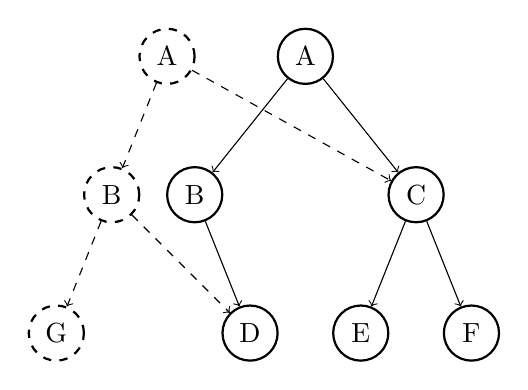
\begin{tikzpicture}[
			oldnode/.style={circle, draw=black, thick, minimum size=7mm},
			newnode/.style={circle, thick, draw=black, dashed, minimum size=7mm},
			]
			\node[oldnode] at (0,0) (root) {A};
			\node[oldnode] at (-4em,-5em) (beta) {B};
			\node[oldnode] at (4em,-5em) (gamma) {C};
			\node[oldnode] at (-2em,-10em) (delta) {D};
			\node[oldnode] at (2em,-10em) (epsilon) {E};
			\node[oldnode] at (6em,-10em) (zeta) {F};
			\node[newnode] at (-5em,0) (newroot) {A};
			\node[newnode] at (-7em,-5em) (newbeta) {B};
			\node[newnode] at (-9em,-10em) (newvertex) {G};
			\draw[->] (root) -- (beta);
			\draw[->] (root) -- (gamma);
			\draw[->] (beta) -- (delta);
			\draw[->] (gamma) -- (zeta);
			\draw[->] (gamma) -- (epsilon);
			\draw[->,dashed] (newroot) -- (gamma);
			\draw[->,dashed] (newroot) -- (newbeta);
			\draw[->,dashed] (newbeta) -- (newvertex);
			\draw[->,dashed] (newbeta) -- (delta);
		\end{tikzpicture}
		\caption{Path copying}
		A new vertex G was added to the structure with solid vertices. Dashed vertices were created by the update -- path from G to the root. Dashed A is the new root.
	\end{center}
\end{figure}

\section{List Ordering}

Moving from semi-persistence to full-persistence we encounter an obstacle -- versions no longer form implicit linear order. (By versions we mean states of the tree in between updates. We will also use some auxiliary versions not directly mappable to any such state.) Nonetheless, to work with fat vertices, we need to be able to determine slots that carry values correct for current version. To achieve this, we need to identify an interval of versions the current vesion would fall into. For this purpose we will try to introduce an ordering to versions of the persistent data structure.

Version do form a rooted tree with the original version in the root. We can also order children of every vertex by the order of their creation (latest creation first). We then define the desired ordering as the order of vertices corresponding to versions as they are visited by an in-order traversal. %TODO: Reformulate in-order.

In reality, we will also insert other elements into the ordering that will be helper version and will not be used to represent the state of the entire structure after a sequence of operations. This can be disregarded for now.

With the ordering defined, we still need a way to efficiently represent it in memory. The operations we really need are two:

\begin{itemize}
	\item \texttt{InsertSuccessor(Version)} -- this operation will insert a new version between \texttt{Version} and its successor (if any). The newly created version is returned.
	\item \texttt{Compare(VersionA, VersionB)} -- returns 1, $-1$, or 0 indicating whether \texttt{VersionA} precedes, succeeds, or equals \texttt{VersionB}.
\end{itemize}

We will strive to find a way to assign an integer to each version, these integers will be comparable in constant time. This assignment problem is called \emph{list-labeling} and there are several options to tackling it.

The straight-forward idea would be to assign 0 to the first version and $2^m$ to an artificial upper bound. All newer versions will be assigned the arithmetic average of its successor and predecessor. Now, we see that if $v = (p + s)/2$ and $ 2^k \mid p, s$, then $2^{k-1} \mid v$. The first two integers are divisible by $2^m$ guaranteeing capacity $\Omega(m)$. 

Let us denote the total number of updates to the persistent tree as $n$. It would be reasonable to  assume that arithmetic operations on non-negative integers less than or equal to $n$ can be done in constant time. We are therefore permitted to create only \bigO{\log n} versions using the straight-forward idea if constant time per operation is needed. This is not sufficient.

To preserve the speed of semi-persistence, \texttt{Compare} must be \bigO{1} and \texttt{InsertSuccessor} \bigO{\log n} at least amortized. Weight-balanced trees that were introduced in the previous chapter are ideally suited for this purpose.

For every vertex in the weight-balanced tree, we will store encoding of the path from root to it in form of sequence of 0s and 1s. 1 for right child, 0 for left child. We know that depth of the tree must be logarithmic, compared integers are composed of \bigO{\log n} bits, so comparison of versions is efficient. Inserting a successor version is also simple. Rebuilding of some subtree will not change order of versions as all path encodings will be recalculated.

Before moving to the next section, we remark that it is possible to get \bigO{1} amortized complexity for insert and delete with weight-balanced trees via indirection as described by Tsakalidis \cite{list-ordering}.

\section{Fully-Persistent Trees}

Before delving into the details of modified fat vertices for full-persistence, we must note that amortized constant number of changes per operation will no longer suffice. If there exist a version of the structure and an operation that causes large amount of changes to the structure, nothing is stopping us from repeatedly performing the operation on that version, thus consuming super-linear amount of space, (Potentially even time complexity may increase.)

To achieve full persistence, we will build upon the technique of fat vertices from previous sections. Now however, simply allocating new vertex when we run out of empty slots in the old one will not do. It remains crucial that occupied slots of one fat vertex form an interval of existing versions. In particular, It will be needed to insert between existing versions.

A new maximum size $m$ of fat vertices will have to be set. If $p$ is the number of pointer fields in original vertices and $k$ the number of required inverse pointers, we set $m = 4(p+k+1)$.
When searching a fat vertex, the slot that applies has the greatest version not exceeding the version that is currently being searched for.

A process modifying the BST data structure may be broken down into a series of updates that only change one vertex or insert a new one. A deleted vertex is not reachable from the root, but technically still exists.
Every such update of the data structure will produce a new version (more than one actually). Since were are only interested in the versions that are associated with the modification that completed an operation on the data structure, existence of other versions can be safely ignored. The total number of versions created will still be in linear with the number of total operations, preserving time complexity.

The process of performing one update involves first of all locating the slot that will be updated. If there exists a slot with the exact same version $v$, it will be updated. Otherwise the slot $s$ corresponding to $v$ is located and copied twice, creating slots $s'$ and $s''$. Slot $s'$ is given the version $v$ and $s''$ a newly created version that succeeds $v$. Then values in $s'$ are updated.
If the update is insert, a new fat vertex with one slot is created instead and its field and pointer values are initialized.

If the current fat vertex has exceeded the number of permitted slots, we add it to a list $l$.
Now inverse pointers must be set in other fat vertices. Similarly, if a slot matching the version is already present in other fat vertex, modifications are applied to that slot. Otherwise two other slots are inserted just as already described. In addition, we add any of the fat vertices where inverse-pointers were updated and slot-capacity exceeded to the list $l$.

The phase of invariant maintenance follows. While $l$ is nonempty, we take a fat vertex $f$ with the highest size from it, check that the number of slots it contains exceeds the limit and then split the node in two. This involves allocating a new fat vertex $f'$ and placing half of the slots with higher half of versions in it. After this split, another pointer check is needed. For versions in the higher half of slots (now slots of $f$), regular and inverse pointers must be checked. For every slot in other fat vertex corresponding to a version belonging to $f'$  that has pointers to $f$, these must be changed to $f'$. 

One slight problem with this splitting is that an interval of versions in some other vertex might intersect a version from both $f$ and $f'$. We know however, that this overlapping can only happen for vertices pointed to by both the slot with greatest version in $f$ and lowest version in $f'$. To remedy this, an extra slot must be inserted to $f'$ bearing a version $h'$ created as successor of $h$ maximum version in $f$. The slot for $h'$ must have fields and pointers initialized with values valid for $h$.

Naturally, creation of this extra slot must be reflected in fat vertices that pointed to $f$ and have an interval now containing $h'$ -- a slot with version $h'$ must be inserted and point to $f'$ instead. Insertion of these extra slots may cause the permitted number of slots to be exceeded in additional vertices and if that is the case, these must be appended to $l$.

It can be clearly seen that this splitting process takes only constant amount of time. When one splitting is complete, another fat node is taken from $l$ and split until it becomes empty.

Avid reader may have noticed a crucial presupposition in this splitting procedure. When a fat vertex is split, its slots must fit into the fat vertices created by that splitting. This is indeed true.

Consider a vertex is split at least twice during one update procedure. Let us take first such a vertex $u$. Before the update started, the number of slots in $u$ definitely had not exceeded capacity. We now try to find an upper bound on the number of new slots inserted into $u$ or its two parts after the first splitting.

Two slots might be inserted due to the actual changes. One slot may be needed for splitting of $u$.
Every other splitting of a fat vertex pointing to $u$ or one of its halves may create up to two new slots (either no slot, a slot in $u$, a slot in one of $u$'s parts, or one slot in both parts). 
Either way, the number of inserted slots is not high enough to trigger another splitting. We therefore reach a contradiction -- no fat vertex can be split more then once. Hence capacity may only be exceeded by a constant amount small enough that after splitting, size invariant holds for the two halves.

Now it is in order to show that $l$ will eventually become empty and what the time complexity is.

\begin{prop}
Starting with an initially empty fully-persistent binary search tree data structure (as described above), a sequence of $n$ updates produces a data structure taking \bigO{n} space while taking \bigO{n \log n} time.
\end{prop}

\begin{proof}
Let us define a potential function for a persistent BST as the sum over all fat vertices of that structure of the number of occupied slots above $3m/4$. Initially the potential is zero and may never be negative. Every update will be charged $m/2 \in \mathcal{O}(1)$ units of energy.

During the first phase, i.e. writing actual changes in the tree to one node, at most $m/2$ extra slots become occupied, these are charged on the update.

During the phase when $l$ is processed, let us have a fat vertex $f$ in $l$. If the size of $f$ is exceeded we must allocate a new fat vertex $f'$. Distributing slots between the two vertices decreases potential by a least $m/4$. We use 1 unit to pay for the new allocation and the remaining units to pay for increase in potential during the check for (inverse-)pointer validity, that is inserting of slots. This implies that potential of the data structure decreases by at least 1 for each splitting in the phase of $l$ processing.

From this argument we also see that the number of node-splitting occurring during one update is limited by the amount of potential available at the start of that update, so it must come to an end.

Every action is now accounted for and the proof is complete.
\end{proof}

\begin{cor}
A sequence of any $n$ tree-operations and $q$ queries on a fully persistent WAVL tree (initially empty) produces a data structure which consumes \bigO{n} memory and takes \bigO{(n+q) \log n} time.
\end{cor}

We should note that the size of vertices is so large, because we did not place any constraint on what updates are allowed to change. If update is only able to change one pointer field for example, we could reduce the size significantly. This would need to be analysed separately for each data structure.

%\begin{prop}
%Suppose any order of splitting fat vertices with the number of slots exceeding the set limit $l$ %during an operation on a tree $T$. Regardless of the way for choosing the next node to be split, %number of occupied slots in all nodes will remain under .
%\end{prop}

\section{Alternative Constructions}

In the previous section, we described fat nodes, where every slot bears all information about the tree vertex. There are other possibilities.

As was already mentioned, we may choose to have a set of default values for all fields and pointers.
These would be initialized to the first version in that fat vertex. Changes would then be stored in form of ordered triples. First would come version, second field or pointer identifier, and last the actual new value. Changing some information by adding a version thus means identifying what are the relevant values first and then inserting update triples.

Yet another option is similar to the last one with the difference that only updates of pointers are allowed. If field needs to be changed, new fat vertex must be allocated.

It is difficult to decide which of these constructions is superior. Complexity will vary for each data structure, ratios between different operations, and other factors.

Finally, let us conclude this chapter with a remark that this approach may be generalized further beyond binary search trees to other pointer-based data structures provided that the constraint on number of pointers targeting one node simultaneously applies to them.
We do not give more attention to such structures in this thesis.


\chapter{Applications of Persistence}

Some of the examples may have more elegant solutions using a different approach. Here the goal is to present the kind of problems where persistence may prove useful and help develop reasoning needed to see other applications should they be encountered by the reader.

\section{Point localization in a plane}

Given a bounded connected subset of a plane partitioned into a finite set of faces, the goal is to respond to queries asking to which face a point $P$ belongs. We limit ourselves to polygonal faces.
One special case of particular importance of this problem is finding the closest point, i.e. when the faces are Voronoi diagrams.

To build the data structure we will follow a general idea of line-sweeping. We start by sorting vertices of all faces by the first coordinate. We will continually process these vertices in the order of increasing first coordinate. We maintain a sorted list of edges (in a semi-persistent BST) during this processing. The list contains edges that intersect with a sweeping-line parallel to the secondary axis in order of the intersections (sorted by the second coordinate). 

Initially the list is empty and we set the sweeping line to intersect the first vertex.
When we start processing a new vertex we imagine moving the sweeping line along the primary axis to intersect with the new vertex. We can easily observe that the order of edges cannot change during this virtual movement. (None of the edges can intersect except in a vertex.) It will happen, however, that edges must be either removed from the list or added to the list. When adding 

We store pointers to the versions created in each in vertex in a sorted array.

The number of vertices will be denoted $n$, the number of edges is thus bounded by $3n$. This follows from the partitioning being drawing of a planar graph. Complexity is therefore \bigO{n \log n} for pre-processing and \bigO{\log n} for one query.

Similar geometric applications of partial-persistence were investigated by Cole \cite{geometric-applications}.


\section{Two-dimensional prefix interval listing}

This application assumes a finite set of $n$ points in a two-dimensional plane. The request is to construct a data structure which could answer queries of the following kind: List %(the number of)
all points $(x_i,y_i)$ satisfying $x_i < \bar x$ and $ y_i \in (\underset{\bar{}}{y}, \bar y) $.

The first step in building data structure for these queries is to sort given points by $x$ coordinate. Then we proceed to add all points in order of increasing $x$ coordinate into a semi-persistent binary search tree. To answer a query with the same parameters as above. We first find a version of the BST where the point added is the greatest lesser than $\bar x$ using binary search on the versions. Then we search that version of the BST and list all points in the specified interval.

With efficient implementation (as discussed in previous chapters), we get \bigO{n \log n} time to prepare the data structure, \bigO{\log n + f} time to answer a query where $f$ points are reported, and asymptotically linear memory consumption. The space requirement is an improvement over range trees\cite{range-trees}.

This data structure can be used as an interval tree by looking at the difference between queries for two different $\bar x$ with the same range for $y$. %TODO: Make more efficient.


\section{???}

Imagine a version control system is used in a repository with branching history. Each version is stored as a patch to another parent version. Now persistent binary tree could be used for queries of files by the last time of modification in history of that particular version.

\section{Binary search in a tree}

Assume we have a rooted tree $T$, totally ordered set $S$ and a function $f: V(T) \rightarrow S$ satisfying that for every vertex $v$ and every ancestor $w$ of $v$ it holds $f(v) \leq f(w)$. 

% f is evaluated in constant time.

We would like to quickly answer large number of queries of the following kind: For given $s \in S$ locate an ancestor $w$ of a vertex $v$ such that $f(w) \leq s$ and for every ancestor $u$ of $w$ it holds that $f(u) > s$. (There is obviously at most one suitable vertex $w$.)

We will build a data structure based on semi-persistent binary search tree which will enable answering this kind of queries in \bigO{\log n} where $n$ denotes the number of vertices of $T$.

The first step is numbering vertices of $T$ by in-order traversal. Next, we construct a structure to answer LCA queries on the tree. %reference?

Now we will finally start building the semi-persistent tree. We add numbers assign to the vertices of $T$ in order of decreasing value of $f$. This involves sorting the vertices by value of $f$ and we store this sorted array for future use. Vertices in the semi-persistent tree are ordered by the assigned numbers. This is the entire preparation phase which takes \bigO{n \log n} time. The structure requires only \bigO{n} memory to store.

In order to locate vertex $w$ for given $v$ and $s$, we locate the version of the semi-persistent tree with all vertices that have value of $f$ grater than $s$. This is done by binary search in the sorted array of vertices. Once the correct version is found we find lower bound and upper bound of $v$. One of these vertices must an ancestor of $v$. This can be verified with the help of LCA structure. If both of those vertices are ancestors of $v$, we take the one further from root. 

We have now located the last ancestor of $v$ with value of $f$ greater than $s$. One of its children must be the queried vertex.

Other solution without employment of persistence could be e.g. with the help of heavy-light decomposition. This would incur a slowdown to \bigO{n \log ^2 n} though.

\section{Dynamic binary search in a tree}

In the previous example we considered that the tree $T$ where queries would be conducted would be static. With full persistence we can afford to add vertices. % remove?

Let $m$ denote the total number of vertices added to the tree.

We will maintain a fully-persistent balanced binary search tree $P$ with vertices ordered by values of $f$. When we want to insert a vertex $z$ to $T$, we also add this vertex to the version of $P$ which was created by adding the parent of $z$. This insert will thus cost \bigO{\log m}.

A query with $s \in S$ and $v \in V(T)$ is simply answered by a search in $P$ in the version created by adding $v$ to $T$. Complexity will be \bigO{\log m}.

Deleting leaves is easy -- no actual procedure is needed. Support for deletion of non-leaf vertices $z$ from $T$ can also be added. Precisely that means that all children of $z$ become children of parent of $z$. (For simplicity we will assume that root will never be deleted, which is a reasonable assumption as an extra root can be added.) 

Vertices are placed into a disjoint-find-union data structure. When a vertex is deleted, it is united with its parent in this data structure. It can be seen that every component in the DFU has a unique root. When searching through $P$ instead of using values of vertices directly, we search the DFU and use vertex found as root of component in the DFU.

This clearly does not break the ordering of vertices in $P$, as there are no possible keys between those of a vertex and its parent for every version. 
 
Not to store excessively many deleted vertices in $P$ and the DFU, we rebuild the entire data structure from the latest version of $T$ when the amount of deleted vertices reaches at least half of the total amount of vertices. The cost to rebuild the tree is obviously amortized into a constant per delete.
 
Depending on the ratio between types of operations, complexity of the queries may be increased. %TODO: Is this amortized completely?

Alternatively, this problem may in addressed by adding a few extra operations to link/cut trees\cite{link-cut}.

%TODO: Look up more examples from articles.

\chapter{Notes on Implementation}

To state the algorithms described in more exact manner the author implemented alternative balancing for WAVL-trees and persistent WAVL-trees as an attachment to this thesis. The format chosen was C\# libraries for .NET Standard platform.

%TODO: Lincense

The goal of the implementation is solely to provide additional clarity into the algorithms. No special optimization has been carried out as this would likely only hinder understanding. It is not intended that someone would include the library in own project, nonetheless that is also possible.

\chapter*{Conclusion}
\addcontentsline{toc}{chapter}{Conclusion}

We introduced a family of binary search trees called rank balanced trees as a useful abstraction and a foundation for Weak AVL trees. Interesting properties of WAVL trees were discussed.

We modified Weak AVL trees to only require a constant number of change per operation (preserving their structural properties). This construction is not known to have been discovered earlier.

We reiterated a general process described by Driscoll et al.\cite{persistence-DSST} for making pointer data structures persistent. The described process was applied to obtain fully-persistent WAVL trees through our modification of that BSTs. Exemplar implementation was provided.

Driscoll et al. used \textit{displacement paths} to deamortize time complexity of insert and delete operations for fully-persistent 2-3 trees. It remains to investigate the possibility of worst case time complexities per operation for WAVL trees. A technique alike that used for 2-3 trees might be used.

Finally some applications of persistence were mentioned.

%%% Bibliography
\include{bibliography}

\appendix
\chapter{Attachments}

\section{Standard Operations}

\begin{algorithm}
	\small
	\SetAlgoLined
	\KwResult{$v$}
	$v \gets $ root of Tree\;
	\While{$v \neq \Lambda$ }{
		\If{Key = $\keyit(v)$}{
			\textbf{halt}\;
		}
		\eIf{Key $> \keyit(v)$}{
			$v \gets \rightit(v)$\;
		}{
			$v \gets \leftit(v)$\;
		}
	}
	\caption{Find(Tree, Key)}
\end{algorithm}

\begin{algorithm}
	\small
	\SetAlgoLined
	$v \gets $ root of Tree\;
	$w \gets \Lambda$\;
	\If{$v = \Lambda$}{
		Create new vertex with Key and Value and set it as root of Tree\;
		{\bf halt}
	}
	\While{$v \neq \Lambda$ }{
		$w \gets v$\;
		\eIf{Key $> \keyit(v)$}{
			$v \gets \rightit(v)$\;
		}{
			$v \gets \leftit(v)$\;
		}
	}
	$u \gets $ new vertex with Key and Value\;
	\eIf{Key $> \keyit(w)$}{	
		$\rightit(w) \gets u$\;
	}{
		$\leftit(v) \gets u$\;
	}
	Rebalance Tree according to chosen algorithm.
	\caption{Insert(Tree, Key, Value)}
\end{algorithm}


\begin{algorithm}
	\small
	\SetAlgoLined$v \gets $ root of Tree\;
	$w \gets \Lambda$\;
	\While{Key $\neq \keyit(v)$ }{
		$w \gets v$\;
		\eIf{Key $> \keyit(v)$}{
			$v \gets \rightit(v)$\;
		}{
			$v \gets \leftit(v)$\;
		}
	}
	\If{$\rightit(v) = \Lambda$}{
		Replace $v$ by $\leftit(v)$ as child of $w$ (if $w$ is internal vertex)\;
		Delete $v$\;
		{\bf go to} 34
	}
	\If{$\leftit(v) = \Lambda$}{
		Replace $v$ by $\rightit(v)$ as child of $w$ (if $w$ is internal vertex)\;
		Delete $v$\;
		{\bf go to} 34
	}
	$x \gets \leftit(v)$\;
	\If{$\rightit(x) = \Lambda$}{
		$ \leftit(v) \gets \leftit(x) $\;
		{\bf go to} 32
	}
	$y \gets \Lambda$\;
	\While{$x \neq \Lambda$}{
		$y \gets x$\;
		$x \gets \rightit(x)$\;	
	}
	$\rightit(y) \gets \Lambda$\;
	Swap keys and values of $v$ and $x$\;
	Delete $x$\;
	Rebalance Tree according to chosen algorithm.
	\caption{Delete(Tree, Key)}
\end{algorithm}

\openright
\end{document}
